\section{EinwegGleichrichter}
Ziel des Versuchs ist es, die Funktionsweise des Einweggleichrichter n\"aher zu bringen. 
\subsection{Experimentelle Durchf\"uhrung}
Die Schaltung wird wie in Abbildung 6 dargestellt, auf dem Steckbrett aufgebaut. Dazu wird eine Siliziumdiode mit einer Durchlassspannung U$_F$ $=$ 0.7~$V$ und ein Widerstand R$_1$ $=$ 1~$k\Omega$ verwendet. Eine sinusf\"ormige Wechselspannung U$_{ein_{pp}}$ = 5~$V$ mit f $=$ 100~$Hz$ wird an den Eingang angeschlossen. Die Ein- und Ausgangsspannung wird an dem Oszilloskop angezeigt.
\begin{figure}[ht]
\begin{center}
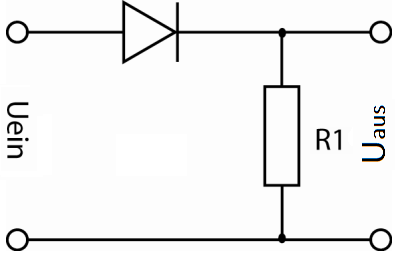
\includegraphics[scale=0.5]{schaltungVersuch2}
\caption{Einweg-Gleichrichter}
\end{center}
\end{figure}
\subsection{Ergebnisse und Diskussion}

Wie in Abbildung 7 zusehen ist werden die negativen Spannungen durch den Einweg-Gleichrichter abgeschnitten. Der Grund hierf\"ur ist, dass die Diode nur in der Durchlassrichtung Strom flie\ss en l\"asst. 
\begin{figure}[ht]
\begin{center}
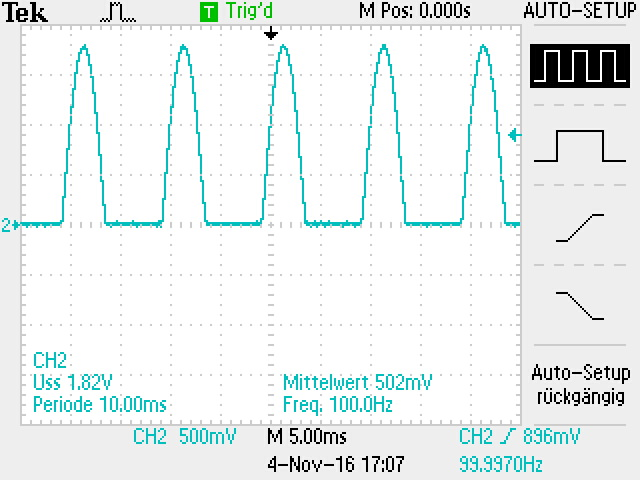
\includegraphics[width=0.5\textwidth]{Bilder/TEK0006}
\caption{Einweg-Gleichrichter}
\end{center}
\end{figure}